\section{Eliminazione di attributi multivalore}\label{sec:multivalue}
L'unico {\it attributo multivalore} presente nel diagramma è l'attributo {\tt Funzione} di {\tt Strumento}
con cardinalità {\tt (1,N)}. Questo attributo può essere facilmente eliminato aggiungendo
una nuova entità {\tt Funzione} legata a {\tt Strumento} tramite una relazione {\it uno-a-molti}
come mostrato in figura:

\vspace{5pt}\centerline{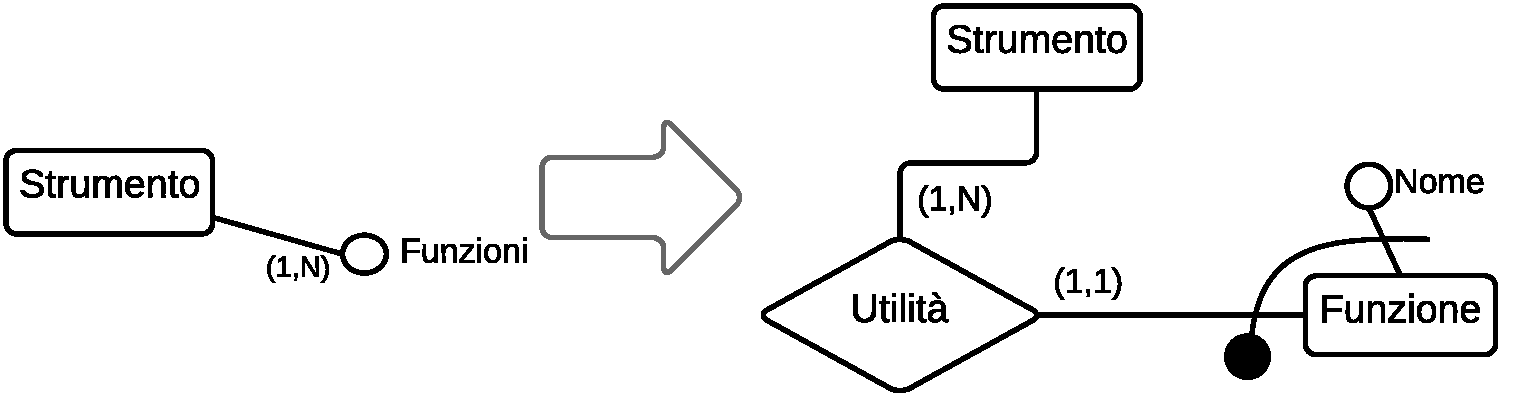
\includegraphics[width=\textwidth]{multi-funzione}}

% TODO: SPIEGARE PERCHÈ ABBIAMO DECISO DI FARE UNA RELAZIONE UNO-A-MOLTI INVECE CHE MOLTI-A-MOLTI
